The final feature extraction code has been run on 483 pictures among which 51 are melanoma, approximately 10\% of the pictures. 

\subsection{{Classifier selection}}
To find the best classifier, first a k-group split was done on the data, to better help avoid over-fitting and to ensure multiple inputs from the same patients stay in the same group. After splitting up the data, we trained and tested our chosen classifiers on each of the groups and took the average of the results to make a final decision on which classifier to use on the entirety of our data set.
\newline
We have tested 3 different types of classifiers, each with different parameters to find the best one from a total of 12 trained classifiers. After calculating a number of metrics, such as accuracy, area under the ROC curve, sensitivity, etc. we gave the highest importance to sensitivity - as melanoma is a deadly condition and it is important to catch all positive cases - together with the F1 score, which is often used for data sets where the classes are imbalanced, just like in our case with only 10\% melanomas in our data set.

\subsection{{Testing classifiers}}
\textbf{The K-Nearest Neighbours} classifier (KNN) is a non-parametric supervised learning algorithm that classifies an instance based on the majority vote of its k nearest neighbors, using distance metrics such as Euclidean or Manhattan distance, from which we have used sickit-learn’s default setting: the Euclidean distance. We have tested this classifier with K set to 1, 3, 5, and 11. K=1 proved to be the most accurate.
\newline
\textbf{Random Forest} is an ensemble learning method that constructs multiple decision trees during training and outputs the mean prediction (regression) of the individual trees. For this classifier we have experimented with changing both the number of estimators used as well as the maximum possible tree height. A total of 7 classifiers were tested with estimator numbers ranging from 100 to 10,000 and the maximum tree heights from undefined to 10. Of all random forest classifiers, the combination of 10,000 estimators and a maximum height of 5 performed the best.
\newline
\textbf{Logistic Regression} is a statistical method for analysing a data set in which there are one or more independent variables that determine an outcome. It is used to model the probability of a binary outcome based on one or more predictor variables. For this classifier we have used all the default settings of sklearn, no parameters were changed.
Out of all trained classifiers, we have picked the Random Forest classifier with number of estimators set to 10,000 and a maximum tree depth of 5, which averaged a sensitivity score of 0.226, a precision score of 0.517, and an F1 score of 0.303 over the five sets of training data.

\begin{table}[!htb] % Use table* to span both columns
    \caption{Aggregated Results of Classifier Training}
    \begin{tabular}{l c c c} % Adjust column alignment as needed
        \toprule
        & \textbf{Sensitivity} & \textbf{Precision} & \textbf{F1} \\
        \midrule
        KNN & 0.249 & 0.235 & 0.233 \\
        RF & 0.226 & 0.517 & 0.303 \\
        LR & 0.082 & 0.400 & 0.122 \\
        \bottomrule
    \end{tabular}
\end{table}

\subsection{{Results from the trained classifier}}
After running the trained classifier on the entire data set of 483 pictures, we have received that 15 out of the 51 melanomas were correctly identified, which leaves us with 36 false negatives, but no false positives. The 100\% precision sounds like a promising result, however, we would sacrifice that for a higher than 30\% sensitivity score, as that is more a relevant evaluation for detecting melanoma.

\begin{figure}[H]
    \centering
    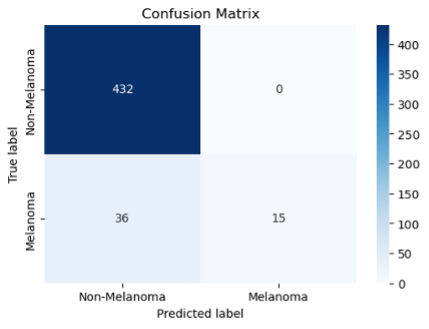
\includegraphics[width=1\linewidth]{ConfusionMatrix.png}
    \caption{Confusion Matrix}
    \label{fig:Confusion Matrix}
\end{figure}